\section{Project timeline: what we planned, what changed, and why}
\label{sec:timeline}

This section tells the story of the project in order. It explains each change of scope and connects each mentor review to what we did about it. The detailed record of individual mistakes is in Section~\ref{sec:mistakes}; here we give the big picture.

\subsection{Week 0: an ambitious proposal}
The Week~0 report (mid-September) was mainly an understanding and related-work document \cite{week0}. It proposed eight components that could each become a service: an authentication service issuing its own tokens, user/profile, organization/tenant, authorization (with a Zanzibar-style ReBAC engine), session and device, SCIM provisioning, consent/audit, and an agent delegation service. Its plan placed most security testing near the end. After a mentor discussion it also added AI agents as first-class principals.

\paragraph{Week 0 review.} The mentor did not object to the problem; the issue was size. Eight independently deployed services would consume the eight-week schedule in networking, deployment and distributed-transaction work instead of in proving security properties. Writing our own OIDC server would be a separate security project. Testing at the end would be too late.

\subsection{Week 1: a precise, smaller design}
The Week~1 design report \cite{week1} kept the security goals and cut the infrastructure:
\begin{itemize}
  \item the eight components became \textbf{modules in one backend} (a modular monolith);
  \item standards-heavy authentication went to an \textbf{existing identity provider};
  \item full SCIM became a \textbf{minimal provisioning slice}, with full SCIM as an extension;
  \item security tests were to be written \textbf{with each milestone}, not at the end;
  \item ten \textbf{security invariants}, a threat model and the first 15 authorization scenarios were written down;
  \item agent identity and delegation stayed in scope as an extension that ``will not be allowed to delay the mandatory M1 to M7 requirements''.
\end{itemize}

\subsection{Week 2: the core system}
By 2 October (commit \texttt{0d232ec}) the core ran in Docker Compose: Keycloak, the Fastify backend with Casbin, PostgreSQL, and browser clients. The suite reported 159 passed tests, and a Playwright script logged in through a real browser with PKCE and through the enterprise broker. Verification uncovered and fixed six integration problems (Section~\ref{sec:mistakes-w2}).

\paragraph{Week 2 review.} The mentor could not open our repository (it returned 404) and found that introspection could be turned off by a flag, that tenant guards were not visibly central, that constants were hard-coded, that some lifecycle assertions were combined, and that we had not shown our tests could fail. The mentor also asked us to freeze our evaluation protocol before Week~3 and asked eight written questions.

\subsection{Week 3: responding, and over-claiming}
On 10--11 October we published the repository, made introspection default-on and fatal to disable in production, added third-tenant and substitution tests, parameterised constants, split the lifecycle assertions, wrote a first ``test-independence'' script and froze the evaluation protocol. The Week~3 report (PDF uploaded 11 October, 11:32 IST, describing commit \texttt{eb50d8b}) presented all of this as done and verified. Two problems were not visible to us yet: some of the new evidence could not actually fail, and the protocol freeze was a day late (Section~\ref{sec:mistakes-w3}).

\paragraph{Week 3 review.} The mentor reran parts of our code and found that the evidence was weaker than claimed: a regression blocked suspended members from withdrawing consent, the mutation script reported success on any error (even with the database stopped), one adversarial test used an ID that could never match, the server answered \code{/health} even with an unsafe configuration, an outage was reported as 401 instead of 503, the hosts were still hard-coded in the client, and M5 lacked a link from a tenant to its email domain and SSO broker.

\subsection{Week 4: rebuilding the evidence}
Before changing anything, we reran the Week~3 head (\texttt{953a0aa}) on a real database: \textbf{160 passed, 1 failed, 6 skipped}. The one failure was the consent regression, which confirmed the mentor's finding and showed that our earlier ``159 passed'' did not apply to the later revision. We then fixed every Week~3 item (commits \texttt{5e4367a}, \texttt{ece833d}, \texttt{42d8a43}) and, for the first time, verified from a \textbf{fresh \code{git clone} with new Docker volumes}: 197 passed, 0 failed, 0 skipped; a rewritten mutation runner killed 7 of 7 injected bugs; the browser proof passed 10 of 10 on two host names. We also corrected two of our own earlier written answers that had overstated what was run. The Week~4 report was completed on 31 October.

\subsection{Week 5: executing our own plan}
No review of the Week~4 report arrived, so in Week~5 we carried out the plan in Section~7 of that report exactly as written. We fixed four dependency advisories that had appeared since Week~2 and one new one (\code{npm audit}: 0). We built AG01, the reporting agent as an application service principal, with the command and expected results stated in advance. We added four mutations, measured latency, and ran the mobile client on a physical Android phone. The clean-clone run of \texttt{fde2efd} on 7 November passed 227 of 227 tests and killed 11 of 11 mutations.

\subsection{Final week: finishing what was promised}
The Week~1 design promised user-to-agent delegation (security invariant~7, scenarios 13 and 14). Every later report listed it as future work. In the final week we built it (AG02, commit \texttt{e13f019}): an assistant agent that can act for a user only through a delegation record bound to one tenant, a list of scopes and an expiry, with permission equal to the intersection of the user's current permission, the delegated scopes and the tenant. We added 26 tests, four mutations, a browser step and a demo script, and reran everything from a clean clone (Section~\ref{sec:results}).

\subsection{Summary of progress}

\begin{table}[H]
\centering
\small
\begin{tabularx}{\textwidth}{@{}P{1.35cm} P{1.6cm} P{1.6cm} P{1.75cm} L@{}}
\toprule
\textbf{Week} & \textbf{Date} & \textbf{Revision} & \textbf{Tests} & \textbf{Main outcome}\\
\midrule
W0 & mid-Sep & --- & --- & Proposal: 8 services, own OIDC server, SCIM, agents\\
W1 & 24 Sep & --- & --- & Modular monolith, Keycloak, Casbin, data model, 10 invariants, 15 scenarios\\
W2 & 2 Oct & \texttt{0d232ec} & 159 / 0 / 0 & Core system, live Keycloak tests, browser PKCE proof\\
W3 & 10--11 Oct & \texttt{eb50d8b} & (not rerun) & W2 review items; first mutation script; protocol frozen one day late\\
W4 start & 31 Oct & \texttt{953a0aa} & 160 / \textbf{1} / 6 & Rerun confirmed the consent regression found by the mentor\\
W4 & 31 Oct & \texttt{42d8a43} & 197 / 0 / 0 & All W3 items fixed; first clean-clone verification; 7/7 mutations\\
W5 & 7 Nov & \texttt{fde2efd} & 227 / 0 / 0 & AG01; npm audit 0; 11/11 mutations; physical phone\\
Final & 14 Nov & \texttt{e13f019} & 253 / 0 / 0 & AG02; 15/15 mutations; 11/11 browser checks on two hosts\\
\bottomrule
\end{tabularx}
\caption{Week-by-week progress. Tests are passed / failed / skipped with real PostgreSQL and the live provider; W2 was run from the build context, W4 onwards from a clean clone.}
\label{tab:progress}
\end{table}

\begin{figure}[H]
\centering
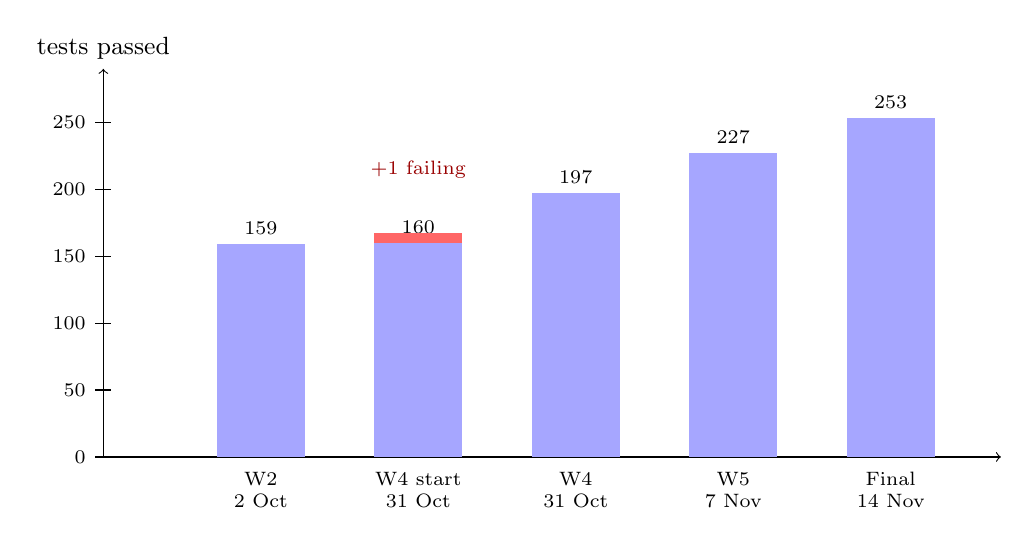
\begin{tikzpicture}[x=2.0cm, y=0.017cm]
  \draw[->] (0,0) -- (5.7,0);
  \draw[->] (0,0) -- (0,290) node[above, font=\small]{tests passed};
  \foreach \y in {0,50,100,150,200,250} { \draw (-0.05,\y) -- (0.05,\y); \node[left, font=\scriptsize] at (-0.05,\y) {\y}; }
  \foreach \x/\v/\lab in {1/159/{W2\\2 Oct}, 2/160/{W4 start\\31 Oct}, 3/197/{W4\\31 Oct}, 4/227/{W5\\7 Nov}, 5/253/{Final\\14 Nov}} {
    \fill[blue!35] (\x-0.28,0) rectangle (\x+0.28,\v);
    \node[above, font=\scriptsize] at (\x,\v) {\v};
    \node[below, font=\scriptsize, align=center] at (\x,-4) {\lab};
  }
  \fill[red!60] (1.72,160) rectangle (2.28,167);
  \node[font=\scriptsize, text=red!60!black] at (2.0,215) {+1 failing};
\end{tikzpicture}
\caption{Passing tests at each verified point. ``W4 start'' is the rerun of the Week~3 head before any fix (160 passed, 1 failed). Mutations killed: none shown at W2, 7 at W4, 11 at W5, 15 at the final run.}
\label{fig:tests-growth}
\end{figure}
